\section{BERT}
\label{sec:bert}
At the start of October 2018 Google published their NLP model called Bidirectional Encoder Representations from Transformers (BERT)~\citep{devlin2018}.
The authors show it is able to score state-of-the-art (SOTA) results for eleven NLP tasks.
A comparison by~\citet{young2018recent} shows ELMo~\citep{peters2018} outperforms various SOTA models on six distinct non-trivial NLP tasks.
The comparison~\citep{young2018recent} continues by showing that BERT gets higher accuracy scores than ELMo for all six tasks.
This by transitivity means that BERT obtains the highest accuracy scores at the time of writing.
BERT being SOTA is also supported by a maintained scoreboard for the Stanford Question Answering (SQuAD) dataset~\citep{rajpurkar2019explorer}.

\subsection{Model description}
\label{subsec:model_description}
% empirical results
Looking into the tasks we see that the results are obtained for a wide range of tasks, including:
\begin{itemize}
    \item Entailment classification.
    For example, ``People formed a line at the end of Pennsylvania Avenue.''
    is contained in (logically implied by) ``At the other end of Pennsylvania Avenue, people began to line up for a White House tour.''~\cite{williams2018}
    \item Semantic text similarity.
    For two sentences determine whether they mean the same thing.
    \item Sentence classification.
    Tasks involve classifying linguistic acceptability (correctness).
    \item Question answering.
    The Stanford Question answering dataset (SQuAD)~\cite{rajpurkar2018} contains questions and a segment of text.
    The answer should be extracted from the segment if it answers the question.
\end{itemize}

% technical description
The paper describes various reasons for the good results on the GLUE, MultiNLI and SQuAD datasets.

% pre-training versus fine-tuning

\subsection{Training}
\label{subsec:training}
% infeasibility of local training
From now on training is used to denote fine-tuning of the model.
Training the general language model on some downstream task is presented as being inexpensive.
Relative to the pre-training it is.
Running training with the advised batch size of 32 will run out of RAM on a 16 GB RAM machine.
The RAM usage on some machine will stay around 15 GB with batch size 16.

To train the model on some tasks it is advised to run `a few epochs'.
Let $a$ be `a few', and $b$ the number of training examples.
Based on the example code provided by Google researchers $a = 3$ and $b = 1000$.
So, it is advised to show the system $3000$ examples.
For our smaller datasets of around 50 examples this means running $3000 / 50 = 60$ epochs.
When measuring the training time in steps it means running $3000 / 16 \approx 188$ steps for a batch size of 16.
Preliminary experiments on the AskUbuntu dataset (having 53 training examples) with a batch size of 32 confirm this estimate, see figure~\ref{fig:tensorboard_base} and~\ref{fig:tensorboard_large_2}.
The images show that the system takes does not easily find a local minimum, and can even have a sudden drop in performance, see figure~\ref{fig:tensorboard_large}.
The results are interesting because it shows that the model is able to learn something even for a dataset with only tens of training examples.
\begin{figure}
    \centering
    \begin{minipage}{0.30\textwidth}
        % \centering
        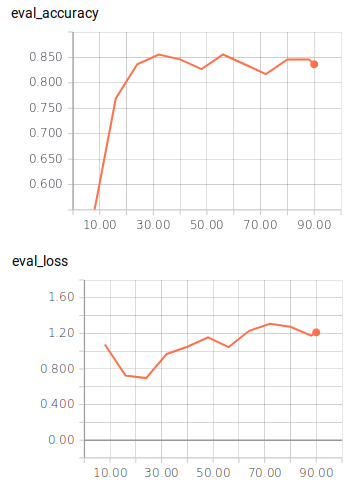
\includegraphics[width=0.9\textwidth]{figures/tensorboard_askubuntu.png}
        \caption{BERT-Base}
        \label{fig:tensorboard_base}
    \end{minipage}
    \hspace*{3mm}
    \begin{minipage}{0.30\textwidth}
        % \centering
        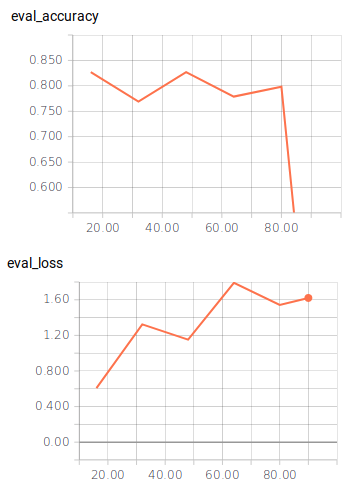
\includegraphics[width=0.9\textwidth]{figures/tensorboard_askubuntu_large.png}
        \caption{BERT-Large}
        \label{fig:tensorboard_large}
    \end{minipage}
    \hspace*{3mm}
    \begin{minipage}{0.30\textwidth}
        % \centering
        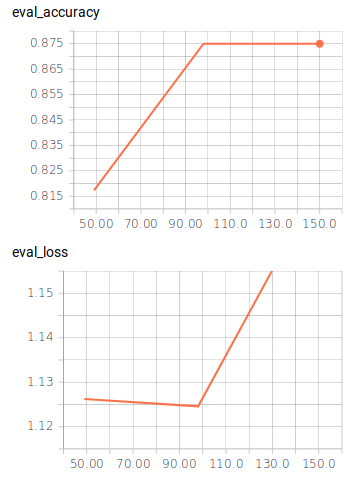
\includegraphics[width=0.9\textwidth]{figures/tensorboard_askubuntu_large_2.png}
        \caption{BERT-Large, second run}
        \label{fig:tensorboard_large_2}
    \end{minipage}

\end{figure}
Training the model for 5 steps or 80 examples takes at least a few hours.
Interpolation suggests that training 188 steps will take at least 36 hours.
This is impractical when doing experiments.

% colab intro
According to the paper the benefit of the Transformer models is that they are highly parallelizable.
Training BERT consist mainly of matrix multiplications~\citep{dettmers2018}.
These can be done quickly and efficiently on graphic processing units (GPUs) and tensor processing units (TPUs).
The latter are ASICs created by Google specifically to do machine learning inference~\citep{jouppi2017}.
When using the TensorFlow implementation of BERT GPUs with 16 GB of RAM are required.
GPU optimizations are available in the PyTorch implementation provided by~\citet{wolf2018}, but this does not support TPUs at the time of writing.
Prices for these GPUs are at least a few thousand euros, which means most users and companies resort to cloud services.
At the time of writing Google Colab (\url{https://colab.research.google.com}) provides free access to a GPU and TPU instance.
One example implementation is provided~\citep{bajaj2018}.

% colab usage
Using Colab is a compromise between usability and costs.
The costs are limited to the use of some storage in a Google Cloud Bucket.
Usability is hindered by the usual constraints of Jupyter Notebooks, for example no unittests, no autocomplete and poor Git integration.
To overcome these issues most of the code is written and tested locally and pushed to a Github repository.
In the Colab the code is then pulled from the repository and main functions are called.
Using Colab has benefits as well.
Hyperparameters and output are visible and can easily be modified in the Notebook, this eases verification.
Reproducibility is possible by opening the Notebook and running all cells.
The first cell will ask to link the Colab to a Google account, make sure this account has access to a Google Cloud Bucket.

% training notes
The plots in figure~\ref{fig:tensorboard_base},~\ref{fig:tensorboard_large} and~\ref{fig:tensorboard_large_2} are created using the default TensorFlow visualisation tool TensorBoard.
Generating these plots can be done by specifying a model and metrics using the TensorFlow Estimator API.

% todo: explain why not listing intermediate accuracies


\subsection{Sentence classification}
\label{subsec:sentence_classification}


\subsection{Joint training}
\label{subsec:joint_training}

% introduction
One reason why neural networks are obtaining the best results for many fields is because networks are now deep.
Deep networks have more layers and can therefore learn more complex tasks.
One application of this is adding a larger portion of some pipeline to the model.
For example, the code by~\citet{rasa2018} for the default pipeline for Rasa Spacy contains the following steps:
\begin{enumerate}
    \item tokenizer
    \item intent entity featurizer regex
    \item intent featurizer spacy
    \item ner crf
    \item ner synonyms
    \item intent classifier sklearn
\end{enumerate}

Training occurs in the ner crf (Stanford Named Entity Recognizer) and intent classifier sklearn component.
For Rasa these two components work separately.
Preferably one would have one model which could learn to do the entire pipeline, also known as an end-to-end model.
It seems unfeasible to train the entire pipeline in a reasonable amount of time.
Using BERT it is possible to train named entity recognition (NER) and intent classification in the same model.

% why it helps
That the combination improves independent models has been shown by~\citet{ma2017jointly} and~\citet{zhang2018joint}.
The results for the former are obtained by using a LSTM network.
The latter introduces an algorithm to combine hidden states from an LSTM.
They show this for the more general problem of sequential labeling and classification.
Intuitively the improvement was to be expected for the following reason.
Suppose we are trying to classify a dataset which contains the sentence:

\begin{center}
    ``I would like to book a ticket to London tomorrow.''
\end{center}

The sentence has intent `BookFlight'.
Training the model could be simplified by providing the sentence classifier with:

\begin{center}
    ``I would like to book a ticket to $<$location$>$ $<$date$>$.''
\end{center}

Now the model does not have to learn to classify sentences while also learning that London is a location and that tomorrow is a date.

% how it should not be done
Note that an end-to-end model is preferred over two separate models.
At the time of writing NER classifiers do not obtain perfect accuracy.
This means that some classifications will be incorrect.
The example from above could instead be converted to:

\begin{center}
    ``I would like to book a $<$date$>$ to $<$location$>$ tomorrow.''
\end{center}

This could make the intent classifier drop in accuracy.
In an ideal end-to-end model incorrect NER classifications would be less of an issue.
The model would learn to ignore the named entity recognition if it would not increase accuracy.



\subsection{BERT joint training}
\label{subsec:bert_joint_training}

% why possible
That joint training BERT is possible can be observed from figure~\ref{fig:bert_single_sentence} and figure~\ref{fig:bert_ner}.
\begin{figure}[htbp]
    \begin{center}
        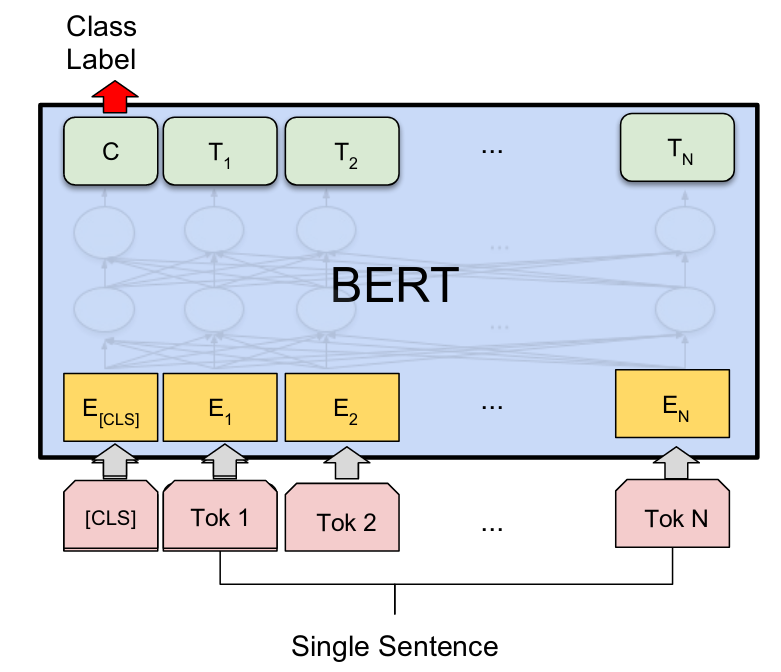
\includegraphics[scale=0.3]{figures/bert_single_sentence.png}
    \end{center}
    \caption{Single sentence classification task~\cite[Figure 3]{devlin2018}.}
    \label{fig:bert_single_sentence}
\end{figure}

\begin{figure}[htbp]
    \begin{center}
        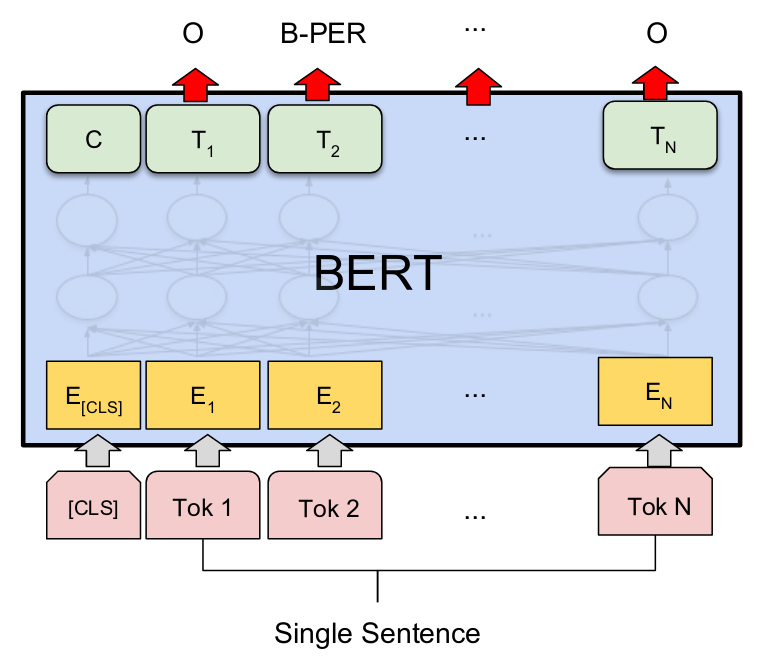
\includegraphics[scale=0.3]{figures/bert_ner.png}
    \end{center}
    \caption{Single sentence tagging task~\cite[Figure 3]{devlin2018}.}
    \label{fig:bert_ner}
\end{figure}

Let $A = A_1, A_2, \cdots, A_n$ denote the layer which is depicted below $C, T_1, \cdots, T_n$, and let $B = B_1, B_2, \cdots, B_n$ denote the layer below $A$.
Let $s$ denote the number of tokens for some input sentence.
By default the max sequence length for the model is set to 128.
For each sentence the sequence length is padded to this max sequence length.
When predicting a `class label' $C$ will only be based on $A_1$ which is based on $B_1, B_2, \cdots, B_s$.
$A_2, A_3, \cdots, A_n$ are not used.
When predicting entities only $A_2, A_3, \cdots, A_s$ are used.
It seems that a joint model is possible by providing the model with a combination of these two.
Consider the NER as a base model and suppose we add some input to $C$.
Now when predicting $C$ the model is expected to learn to look at input from $A$.
For this it can use entity information from $A_2, A_3, \cdots, A_s$.
To also learn non-trivial patterns in non-entity words in the sentence it can use $A_2, A_3, \cdots, A_n$.
Typically sentences are much shorter than 128 tokens so enough space should be available in $A_2, A_3, \cdots, A_n$.
To allow for more space the max sequence length can be increased, this will increase training and inference time.

% how done
To do this the input for the model has been changed from: \\

\noindent \verb|text: ['how', 'do', 'i', 'disable', 'the', 'spam', 'filter', 'in', 'gmail', '?']|\\
\verb|true: ['O', 'O', 'O', 'O', 'O', 'O', 'O', 'O', 'B-WebService', 'O']|\\

to\\

\noindent \verb|text: ['INTENT', 'how', 'do', 'i', 'disable', 'the', 'spam', 'filter', 'in',|\\
\hspace*{12cm} \verb|'gmail', '?']|\\
\verb|true: ['FilterSpam', 'O', 'O', 'O', 'O', 'O', 'O', 'O', 'O', 'B-WebService', 'O']|\\

where `text' is passed to $C, T_1, \cdots, T_s$ and `true' to $E_{[CLS]}, E_1, \cdots, E_n$ during training.
% In the default BERT model $[CLS]$ is passed to denote that the model is used for classification.
The BERT tokenizer splits words which are not listed in the vocabulary corresponding to a pre-trained model.
INTENT is capitalized to force it to be out-of-vocabulary, it is converted by BERT to [UNK].
The goal of this is to avoid overriding the default interpretation BERT has for `intent' (or any other uncased token we choose).

% loss function
The NER loss function can be applied to the joint training without change.
This is counterintuitive because input examples have one position for the class $C$ and $s$ positions for the entities $T_1, T_2, \cdots, T_s$.
Typically sentences have around 10 tokens after tokenization.
So, the loss is based on around one intent position and ten entities.
This means that the model will learn entity recognition much quicker than intent classification.
For situations where the model is able to learn the entities quickly this is not expected to affect the performance of the intent classification significantly.
% explain more
It is expected that the only significant difference of this change is in the difficulty of the loss function.
% explain morec